\subsection{Static predicates}
In this section we define
the static predicates identified in the traffic rules.
The arguments of the predicates are traffic-related objects
such as lane, turn signal, etc.

%--------------------------------
\subsubsection{Intersection lane}
An \emph{intersection lane} is a lane
that connects an incoming lane to an outgoing lane
of the intersection.
A \emph{lane} is a tube-shaped volume
that is curved along its length
and has a rectangular cross section.
The \emph{center} of the lane is a spline curve
along the length of the tube.
The left and right boundaries of an intersection lane
are offsets of the center by half of the lane width.
The \emph{width} of a lane changes
from the width of the incoming lane to the width of the outgoing lane.
This change is linear
with respect to the length of the center curve from the incoming lane.
The bottom of the lane aligns on the pavement.
In Figure \ref{fig:intersection-lane}
we see an example of left-turn,
right-turn,
and no-turn intersection lanes.

\begin{figure}% >>>
  \centering
  \begin{minipage}[t]{.43\linewidth}
    {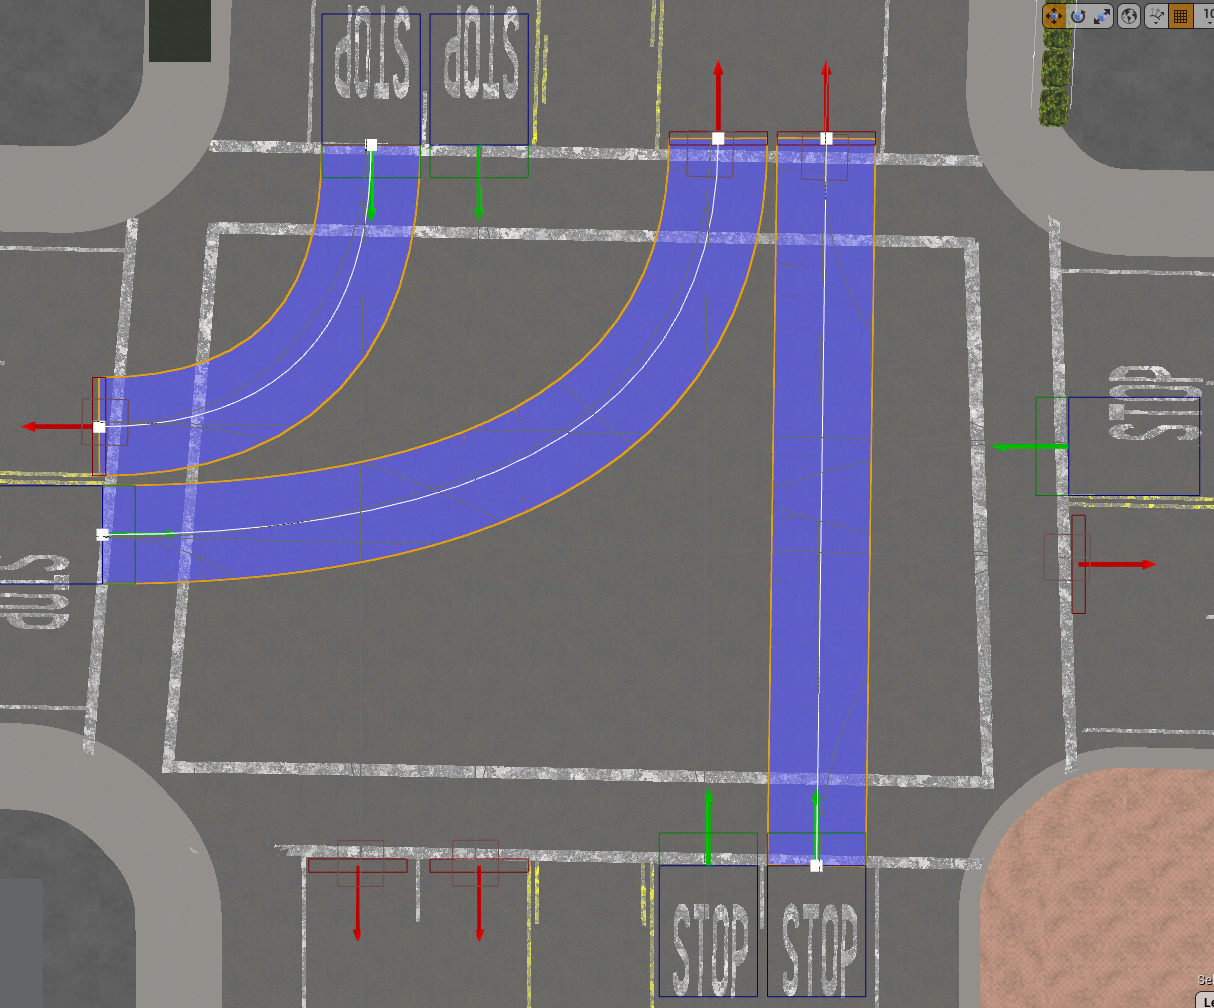
\includegraphics[width=\linewidth]{figures/chapter3/intersection-lane.png}}%
    \subcaption{Top view}
  \end{minipage}%
  \hfill
  \begin{minipage}[t]{.555\linewidth}
    {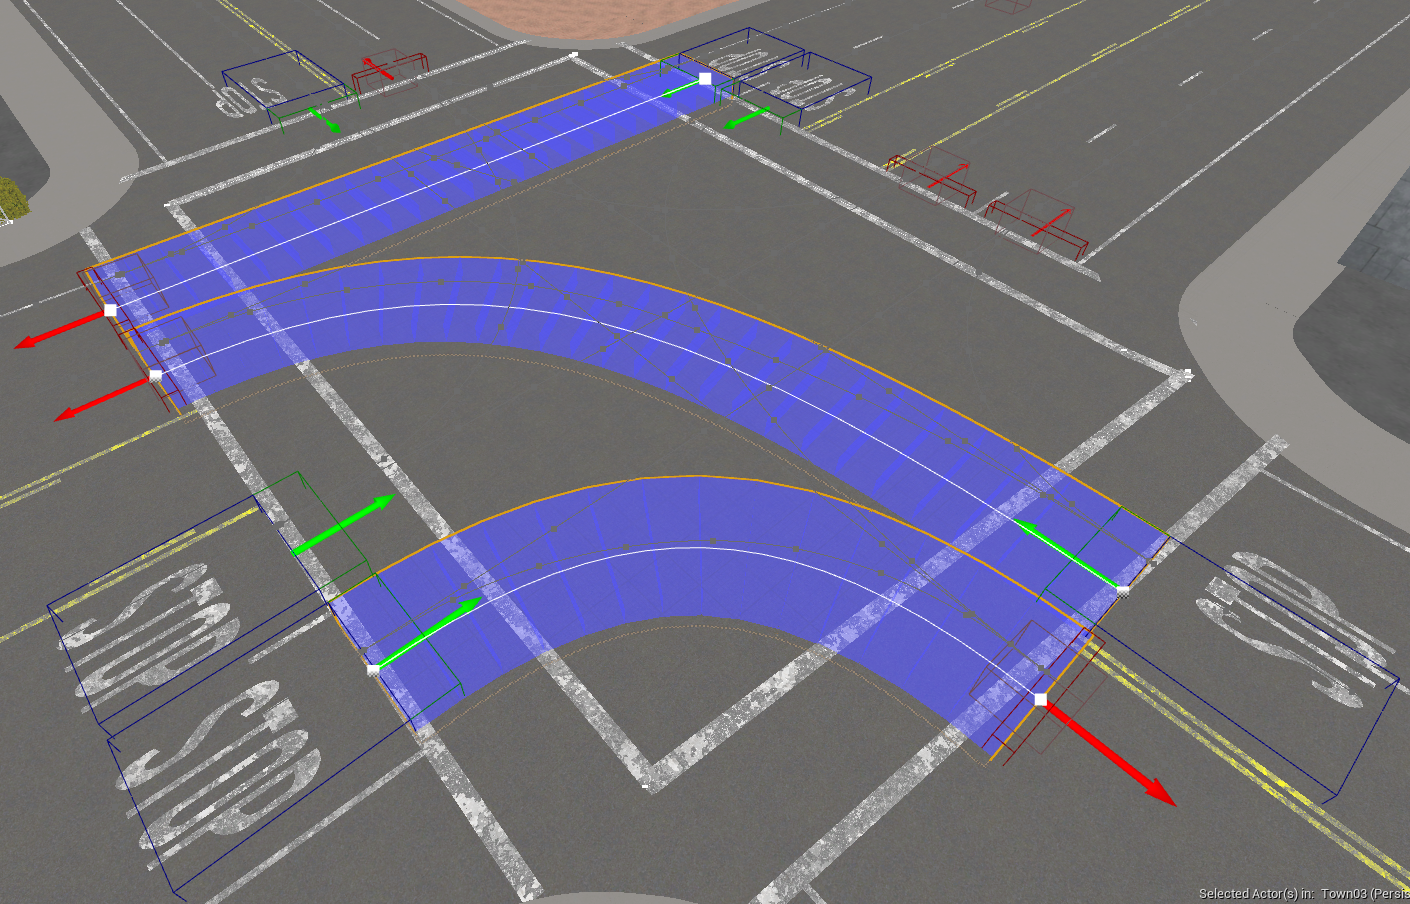
\includegraphics[width=\linewidth]{figures/chapter3/intersection-lane_perspective.png}}%
    \subcaption{Perspective view}
  \end{minipage}%
  \caption{Examples of intersection-lane geometry.}\label{fig:intersection-lane}%
\end{figure}% <<<
%-------------------
\subsubsection{Fork}
A \emph{fork} is the set of
all intersection-lanes that start from the same incoming lane.
Each intersection-lane is called a \emph{branch} of its fork.
Since there is a one-to-one correspondence between forks and incoming lanes,
we can identify a fork with an incoming lane or vice versa.
%--------------------------
\subsubsection{Lane overlaps}
The predicate $overlaps$ holds for a pair of intersection lanes if
their regions intersect.
Therefore, it defines a symmetric relation.
%--------------------------
\subsubsection{Is-on-right-of relation for forks}
We define $isOnRightOf(F2, F1)$ for two forks,
based on their corresponding incoming lanes.
The relation $isOnRightOf$ must be irreflexive and anti-symmetric.\footnote{That is,
no fork is to the right of itself;
and if $F2$ is on the right of $F1$ then
$F1$ is not on the right of $F2$.}
The driver handbook does not give a clear definition.
We define this relation based on angles between vectors.
The direction of an incoming lane
defines a 2D vector on the plane (i.e. the pavement).
We say $F2$ is \emph{on the right of} $F1$ if the angle of $F2$ relative to $F1$,
measured counterclockwise,
is more than 30 and less than 150 degrees.\footnote{The Federal Highway Administration recommends that
``in the design of new facilities or redesign of existing facilities where right-of-way is restricted,
intersecting roadways should meet at an angle of not less than 75 degrees.''\cite{FHWA.2001}
However,
as we see in Figure \ref{fig:on-the-right-of} (c),
the north side of 46th St is 40 degrees to the right of Pico Way.
Therefore,
we choose a conservative infimum of 30 degrees.}
The direction \emph{counterclockwise} is with respect to a downward view of the intersection from above.

For example,
consider Figure \ref{fig:on-the-right-of} (b).\footnote{Intersection of
Harrison Street and Providence Street, Worcester, Massachusetts.}
It shows the incoming lanes
and the angles between consecutive lanes.
Then, as expected intuitively,
the predicate $isOnRightOf$ holds for the following pairs:
$(East, South)$,
$(North, East)$,
$(West, North)$, and
$(South, West)$.
Under our definition,
more than one leg of an intersection may be on the right of another leg.
For example,
consider Figure \ref{fig:on-the-right-of} (c).\footnote{Intersection of
46sth St, F St, and Pico Way, Sacramento, California.}
The F Street and Pico Way are 50 degrees and 140 degrees from south side of 46th Street,
counterclockwise.
Hence, both of them are on the right of (the south side of) 46th Street.
\begin{figure}% >>>
  \centering
  \begin{minipage}[b]{.3\linewidth}
    \subcaptionbox{Definition}
      {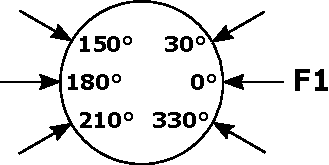
\includegraphics[width=\linewidth]{figures/chapter3/onTheRightOf_Horizontal.pdf}}
    \subcaptionbox{Example.}
      {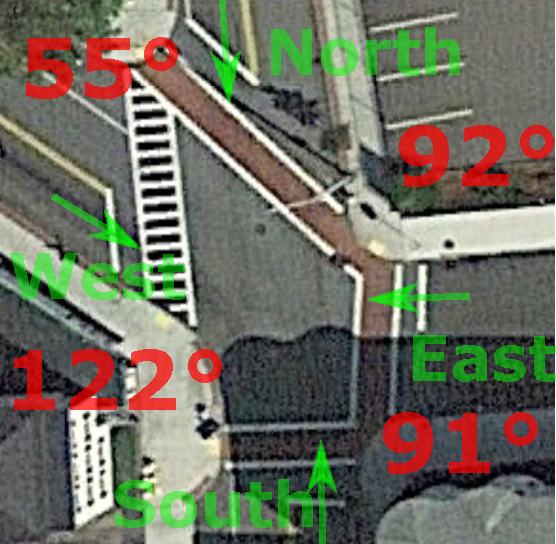
\includegraphics[width=\linewidth]{figures/chapter3/onTheRightOf_Harison-Providence.pdf}}%
  \end{minipage}%
  \hspace*{5mm}
  \begin{minipage}[t]{.3\linewidth}
    \subcaptionbox{Multiplicity}
      {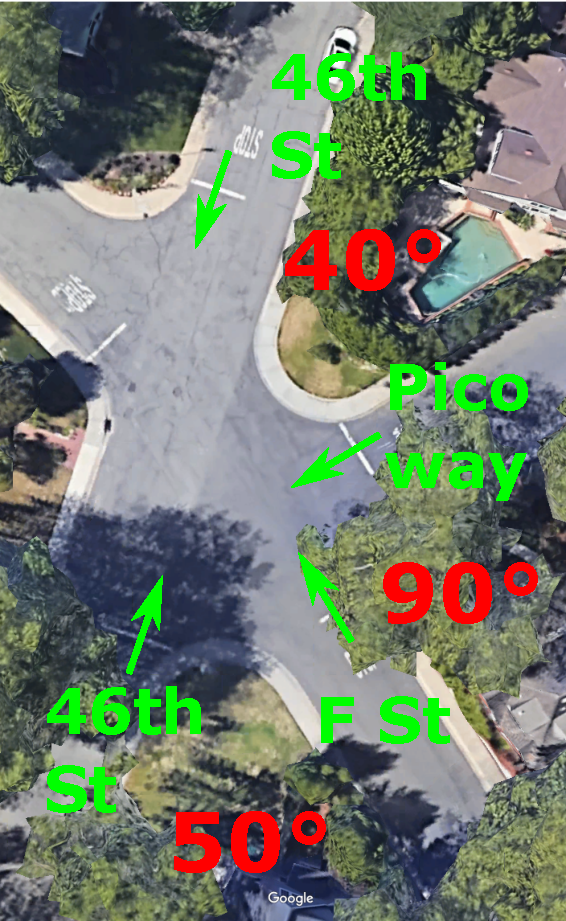
\includegraphics[width=\linewidth]{figures/chapter3/onTheRightOf_F-46th.pdf}}%
  \end{minipage}%
  \caption
  {%
    Is-on-right-of relation for forks.%
    \label{fig:on-the-right-of}%
  }%
\end{figure}% <<<

If the angle from $F1$ to $F2$ is in the interval $[0, 30]$ or $[330, 360)$,
then the incoming lanes are considered heading the same direction,
i.e. on the same street.
If the angle is in $[150, 210]$
we say $F2$ is \emph{in front of} $F1$
i.e. vehicles on $F2$ are \emph{oncoming traffic} relative to $F1$.
If the angle is in $(210, 330)$,
then $F2$ is on the left of $F1$,
i.e. $F1$ is on the right of $F2$.

%--------------------------
\subsubsection{Arrival box}
The \emph{arrival box} is 
a box on an incoming lane that starts at
a pre-specified distance from the intersection (i.e. before the end of the incoming lane)
and ends at the border between the incoming lane and the intersection.
This distance is the \emph{length} of the box.
The \emph{width} of the box is the width of the arriving lane.
The length of the box is a hyperparameter.
For example,
in Figure \ref{fig:arrival-line},
the dark-blue boxes at the crosswalk lines,
designate the boundaries of the arrival box.
In this example,
the length of the box is 4 meters.
When a vehicle overlaps an arrival box,
an arrival event is generated.

\begin{figure}
\centering
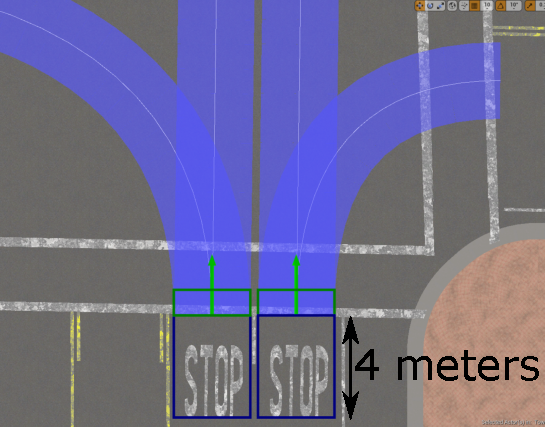
\includegraphics[width=.5\linewidth]{figures/chapter3/arrival-line.pdf}
\caption{Arrival box.}
\label{fig:arrival-line}
\vspace{-0.5cm}
\end{figure}

%--------------------------
\subsubsection{Entrance box}
This box is used to generate the entrance event.
It marks the boundary between an incoming lane and the intersection area.
Each fork has an entrance box.
%--------------------------
\subsubsection{Lane-from-to}
The predicate $laneFromTo(L, F, E)$
indicates that lane $L$ starts at fork $F$ and ends at exit $E$.
Therefore,
this predicate specifies the possible routes through the intersection.
